\documentclass[12pt]{article}
\usepackage[margin=1in]{geometry}
\usepackage{amsmath,amssymb,amsthm,booktabs,graphicx,natbib,microtype,array}
\newtheorem{theorem}{Theorem}
\newtheorem{proposition}[theorem]{Proposition}
\newtheorem{corollary}[theorem]{Corollary}
\newtheorem{remark}[theorem]{Remark}
\newcommand{\smin}{\sigma_{\min}}
\title{Conditional All-Level Reset Dichotomy\\\large Inclusion-Minimal Native and Adaptive-Lag Interfaces}
\author{Prime Dynamics Theory Program}
\date{July 2026}

\begin{document}
\maketitle

\begin{abstract}
The reset program now has two finite survivors but no all-level theorem.  We
turn that boundary into a precise conditional dichotomy.  Let $U_n$ be
rank-$r$ spectral reset frames, $r\geq4$, let $M_n=R_n+T_n$, and denote the
selected full-memory endpoints by $\ell_n,u_n$, a tail-mass upper by $\tau_n$,
and the consecutive frame overlap by $C_n=U_{n-1}^*U_n$.

Three eventual interfaces suffice for a uniform native floor:
\[
 \smin(C_n)\geq a>0,\qquad
 q_n:=\frac{\tau_n}{\ell_n-\tau_n}\leq q<1,
 \qquad
 \delta_n:=\frac{\ell_n-\tau_n}{u_n}\geq\delta>0.
\]
They imply
\[
 \inf_n\mathcal N_n\geq
 a\sqrt\delta(1-\sqrt q)^4>0.
\]
If, additionally, some lag $1\leq k_n\leq K$ has normalized fourth-cross
lower $\sigma_4((I-P_{n-k_n})R_nP_{n-k_n})/\sigma_1\geq b>0$, then the
transported directional seed obeys
$\inf_n\mathcal D_n\geq a^K b>0$.

The native set is inclusion-minimal for this formula; the joint
native--directional set is inclusion-minimal after the lag interface is
split into bounded lag and positive normalized cross.  Explicit witnesses
make each omitted floor tend to zero.  On the frozen atlas every clause
passes.  Independent worst constants give a native floor
$3.0883\times10^{-12}$, while the selected-path directional floor is
$2.1194\times10^{-23}$; replacing selected paths by $a^8$ gives only
$6.0283\times10^{-48}$.  These are finite calibrations, not evidence that the
eventual interfaces hold.  The theorem is a falsifiable roadmap and makes no
Stage A, Hilbert--Polya, zero-identification, or RH claim.
\end{abstract}

\section{The two output types}
Let $P_n=U_nU_n^*$ and compress the full, recent, and tail memories to the
current packet:
\[
 G_n=U_n^*M_nU_n,\qquad H_n=U_n^*R_nU_n,
 \qquad D_n=U_n^*T_nU_n,\qquad G_n=H_n+D_n.
\]
Assume $G_n$ has spectrum in $[\ell_n,u_n]$ and
$0\preceq D_n\preceq\tau_nI$.  The native certificate functional is
\[
 \mathcal N_n=
 \frac{\smin(C_n)}{\sigma_1(C_n)}
 \sqrt{\frac{\lambda_{\min}(H_n)}{\lambda_{\max}(G_n)}}
 \left(1-\sqrt{\|H_n^{-1/2}D_nH_n^{-1/2}\|}\right)_+^4.
\]
It packages transition conditioning, recent spectral spread, and relative
tail loss exactly as in the RH-156 support formula.

For a lag $k$, put $Q_{n,k}=P_{n-k}$ and
\[
 B_{n,k}=(I-Q_{n,k})R_nQ_{n,k},\qquad
 W_{n,k}=C_{n-k+1}\cdots C_n.
\]
The transported directional seed is
\[
 \mathcal D_{n,k}=\smin(W_{n,k})
 \frac{\sigma_4(B_{n,k})}{\sigma_1(B_{n,k})}.
\]
This definition keeps the native and cross types separate.  A later assembly
must declare which one it accepts.

\section{Conditional all-level theorem}
\begin{theorem}[Native--directional reset dichotomy]\label{thm:dichotomy}
Suppose that, for every $n\geq N$:
\begin{enumerate}
\item[\textnormal{(O)}] $\smin(C_n)\geq a>0$;
\item[\textnormal{(E)}] $\ell_n>\tau_n$ and
$q_n=\tau_n/(\ell_n-\tau_n)\leq q<1$;
\item[\textnormal{(S)}] $(\ell_n-\tau_n)/u_n\geq\delta>0$.
\end{enumerate}
Then
\[
 \mathcal N_n\geq
 \mathcal N_*:=a\sqrt\delta(1-\sqrt q)^4>0
 \qquad(n\geq N).
\]

If, in addition,
\begin{enumerate}
\item[\textnormal{(L)}] there are constants $K<\infty$ and $b>0$ such that
for every $n\geq N$ some $1\leq k_n\leq K$ satisfies
\[
 \frac{\sigma_4(B_{n,k_n})}{\sigma_1(B_{n,k_n})}\geq b,
\]
\end{enumerate}
then
\[
 \mathcal D_{n,k_n}\geq\mathcal D_*:=a^Kb>0.
\]
\end{theorem}
\begin{proof}
Since $G_n\succeq\ell_nI$ and $D_n\preceq\tau_nI$,
$H_n\succeq(\ell_n-\tau_n)I$.  Therefore
\[
 D_n\preceq \frac{\tau_n}{\ell_n-\tau_n}H_n\preceq qH_n,
 \qquad
 \frac{\lambda_{\min}(H_n)}{\lambda_{\max}(G_n)}\geq\delta.
\]
Frame overlaps are contractions, so $\sigma_1(C_n)\leq1$ and
$\smin(C_n)/\sigma_1(C_n)\geq a$.  Substitution into $\mathcal N_n$ gives
the native floor.

For the selected lag, least singular values are supermultiplicative:
$\smin(W_{n,k_n})\geq a^{k_n}\geq a^K$.  Multiplication by the normalized
fourth-cross lower $b$ gives the directional floor.
\end{proof}

Condition (E) is the sharp subunit gate: $q<1$ is equivalent to
$\ell_n>2\tau_n$.  Condition (S) is independent; a weak mode and its tail may
decay together so that $q_n$ stays below one while the recent/full normalized
base tends to zero.

\begin{corollary}[Outwardly checkable lag interface]\label{cor:outward}
Let a nominal lagged cross have first and fourth singular values
$\widehat s_1,\widehat s_4$ and certified operator radius $\rho$.  If
\[
 \widehat s_4-\rho\geq\gamma>0,
 \qquad \widehat s_1+\rho\leq\Gamma<\infty,
\]
then (L) holds with $b=\gamma/\Gamma$.  For a Hermitian recent center
$\widehat R$, matrix radius $r_R$, and projector radius $\epsilon$, one may
take
\[
 \rho=r_R+\bigl(\lambda_{\max}(\widehat R)-
 \lambda_{\min}(\widehat R)\bigr)\epsilon.
\]
\end{corollary}
\begin{proof}
Singular-value perturbation gives the first assertion.  The second is the
shift-invariant centered projector-action radius of RH-158
\citep{Bhatia1997,StewartSun1990}.
\end{proof}

\section{Inclusion-minimal interfaces}
The minimality below is relative to the displayed modular functionals, not a
claim that no future construction can bypass them.

\begin{theorem}[Omission witnesses]\label{thm:minimal}
The interface set $\{\mathrm O,\mathrm E,\mathrm S\}$ is inclusion-minimal
for a uniform positive lower on $\mathcal N_n$.  The set
$\{\mathrm O,\mathrm E,\mathrm S,\mathrm L\}$ is inclusion-minimal for the
joint conclusion $\inf\mathcal N_n>0$ and $\inf\mathcal D_{n,k_n}>0$.
Within (L), both bounded lag and a positive normalized fourth-cross lower are
necessary for the stated directional formula.
\end{theorem}
\begin{proof}
Keep all unmentioned interface constants fixed.  Without (O), take admissible
overlap lowers $a_n\downarrow0$.  Without (E), take relative tail ratios
$q_n\uparrow1$ while the recent/full ratio stays bounded below; the fourth
power tail factor tends to zero.  Without (S), take recent compressions with
one eigenvalue $\varepsilon_n\downarrow0$ and tail mass proportional to
$\varepsilon_n$; then $q_n$ remains fixed but $\delta_n\downarrow0$.

Without a positive cross ratio, choose $R_n$ block diagonal relative to every
candidate packet; native positivity can remain uniform while
$\sigma_4(B_{n,k})=0$.  Finally, if only lags $k_n\to\infty$ carry a fixed
cross ratio and $0<a<1$, then the guaranteed transport factor
$a^{k_n}\to0$.  Each proper omission therefore admits a sequence with the
remaining modular interfaces intact and the requested floor vanishing.
\end{proof}

The explicit audit uses indices $1,2,4,8,16,32,64$ for all five witnesses and
checks monotone floor collapse.  These examples mark exact logical failure
modes rather than predicting which one the prime-dynamics sequence will
exhibit.

\section{Finite calibration}
The 120-transition atlas supplies
\[
 a=8.98663\times10^{-5},\qquad
 q=0.2246959,\qquad
 \delta=2.01608\times10^{-13}.
\]
Using independent worst cases in Theorem~\ref{thm:dichotomy} gives
\[
 \mathcal N_*=3.08834\times10^{-12}.
\]
Taking global endpoint extrema rather than the three interface extrema gives
the still more conservative $2.44778\times10^{-12}$; evaluating each
transition locally gives minimum $3.26204\times10^{-8}$.  All are valid finite
numbers with different correlation loss.

For the lag route,
\[
 K=8,\qquad \gamma=3.18077\times10^{-16},\qquad
 \Gamma=0.224446.
\]
The theorem's purely consecutive bound is
$a^8\gamma/\Gamma=6.02832\times10^{-48}$.  The archived selected paths have
common overlap $1.49553\times10^{-8}$, improving the transported floor to
$2.11941\times10^{-23}$.  The minimum local, untransported normalized base is
$2.58742\times10^{-14}$.  The forty-order spread between local and modular
worst-case bounds is precisely the conditioning problem an all-level proof
must address.

\begin{figure}[t]
\centering
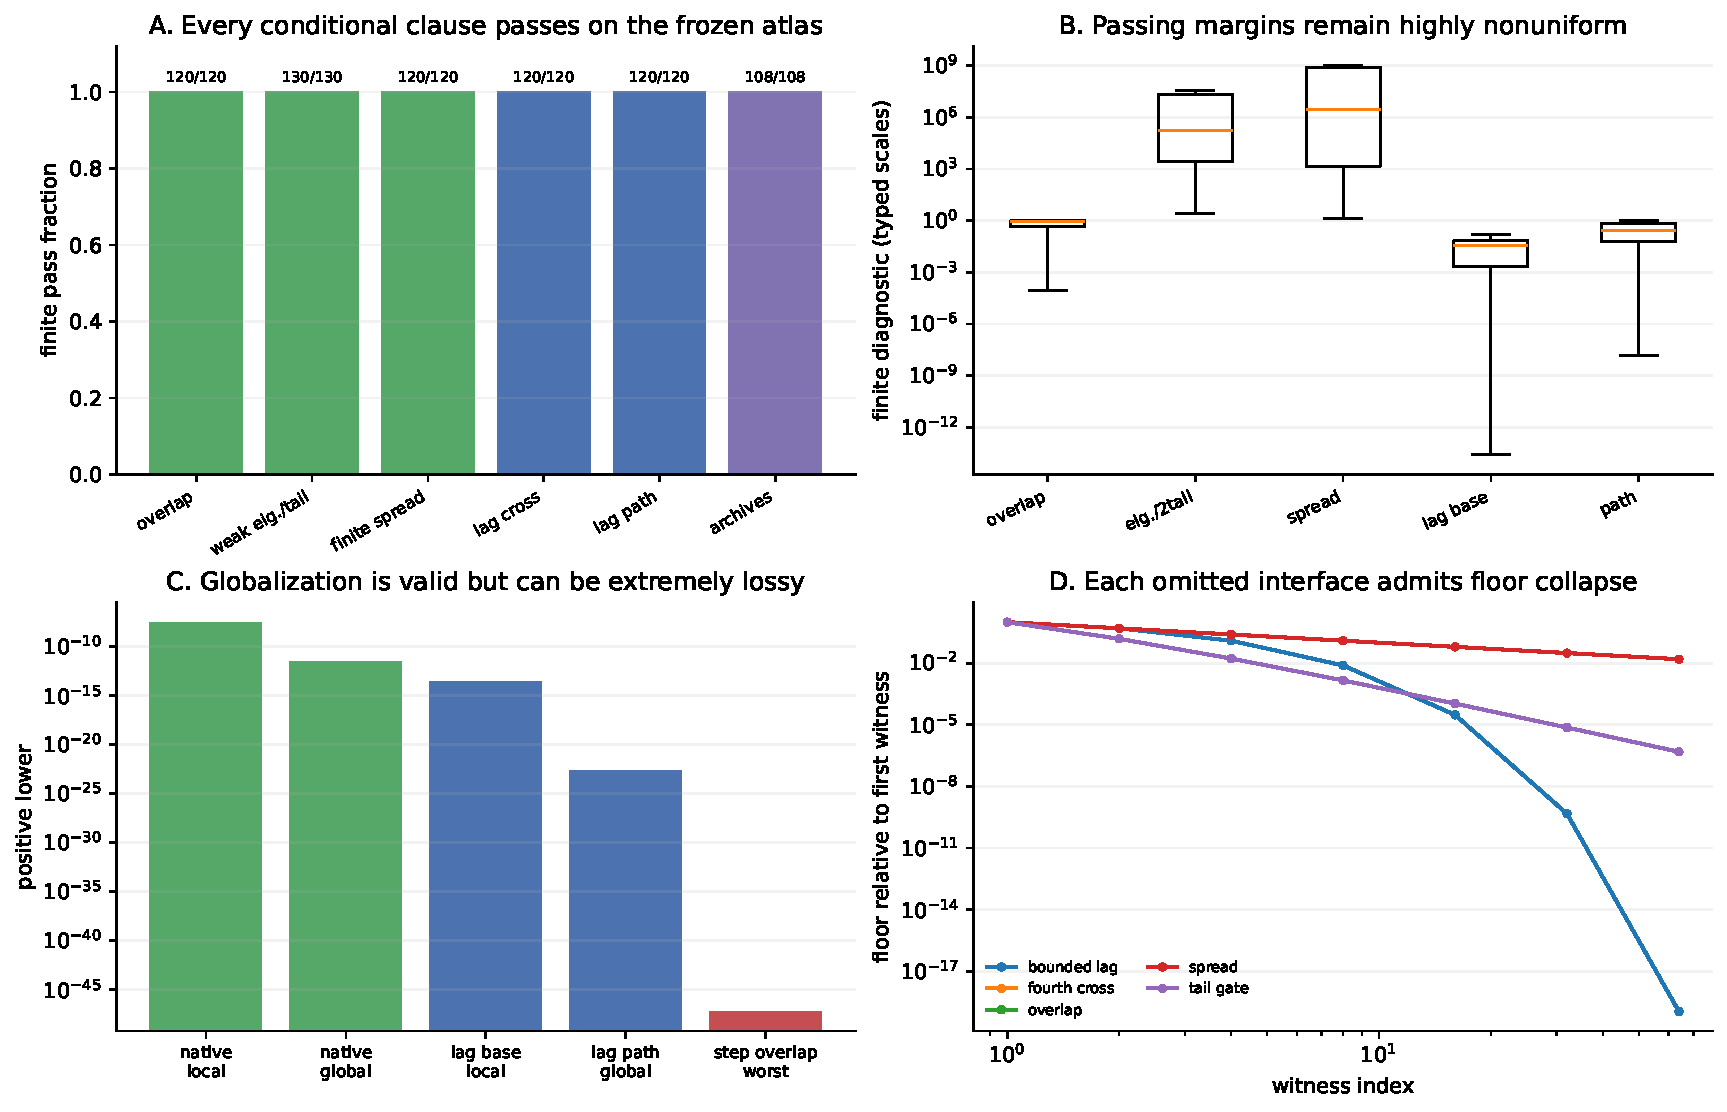
\includegraphics[width=\textwidth]{figures/conditional_all_level_reset_dichotomy.pdf}
\caption{Finite clause audit, nonuniform diagnostics, globalization loss, and
the five explicit omission mechanisms.}
\label{fig:audit}
\end{figure}

\section{Falsifiable roadmap and boundary}
\begin{table}[ht]
\centering
\small
\begin{tabular}{c>{\raggedright\arraybackslash}p{5.0cm}>{\raggedright\arraybackslash}p{7.2cm}}
\toprule
interface & eventual statement & direct falsifier\\
\midrule
O & $\inf\smin(C_n)>0$ & running overlap minimum tends to zero\\
E & $\sup q_n<1$ & weak eigenvalue reaches twice tail mass\\
S & $\inf\delta_n>0$ & selected recent/full ratio tends to zero\\
L & bounded lag and $\inf\sigma_4/\sigma_1>0$ & required lag grows or cross margin closes\\
A & typed downstream assembly accepts the seed & radius overflow or packet-type mismatch\\
\bottomrule
\end{tabular}
\caption{Interfaces and observations that would reject the present route.}
\label{tab:falsifiers}
\end{table}

The next theoretical work is not another large finite count.  It is to derive
scale laws for O, E, and S, then L if the directional output is required.  At
each stage the table supplies a clean negative outcome.  Only after one route
has eventual interfaces should its seed be inserted into a single typed
assembly A.

The archive audit rechecks all 108 publication hashes from RH-151--RH-159;
all match.  RH-160 proves the conditional formulas and their omission
witnesses and calibrates every hypothesis on the finite atlas.  It does not
prove that O, E, S, L, or A holds eventually for the prime-dynamics sequence,
does not close Stage A, does not construct a Hilbert--Polya operator, does not
identify zeta zeros, and does not prove the Riemann Hypothesis.

\bibliographystyle{plainnat}
\bibliography{references}
\end{document}
